%%%%%%%%%%%%%%%%%%%%%%%%%%%%%%%%%%%%%%%%%%%%%%%%%%%%%%%%%%%%%%%%%%%%%%%%%%%%%%%%
%
% Template license:
% CC BY-NC-SA 3.0 (http://creativecommons.org/licenses/by-nc-sa/3.0/)
%
%%%%%%%%%%%%%%%%%%%%%%%%%%%%%%%%%%%%%%%%%%%%%%%%%%%%%%%%%%%%%%%%%%%%%%%%%%%%%%%%

%   PACKAGES AND OTHER DOCUMENT CONFIGURATIONS

\documentclass[
11pt, % The default document font size, options: 10pt, 11pt, 12pt
%oneside, % Two side (alternating margins) for binding by default, uncomment to switch to one side
%chapterinoneline,% Have the chapter title next to the number in one single line
spanish,
singlespacing, % Single line spacing, alternatives: onehalfspacing or doublespacing
%draft, % Uncomment to enable draft mode (no pictures, no links, overfull hboxes indicated)
%nolistspacing, % If the document is onehalfspacing or doublespacing, uncomment this to set spacing in lists to single
%liststotoc, % Uncomment to add the list of figures/tables/etc to the table of contents
%toctotoc, % Uncomment to add the main table of contents to the table of contents
parskip, % Uncomment to add space between paragraphs
%codirector, % Uncomment to add a codirector to the title page
headsepline, % Uncomment to get a line under the header
]{MastersDoctoralThesis} % The class file specifying the document structure

%----------------------------------------------------------------------------------------
%	INFORMACIÓN DE LA MEMORIA
%----------------------------------------------------------------------------------------

\thesistitle{Diseñó de Interfaz Digital Serie para Dispositivo Lógico Programable} % El títulos de la memoria, se usa en la carátula y se puede usar el cualquier lugar del documento con el comando \ttitle

% Nombre del posgrado, se usa en la carátula y se puede usar el cualquier lugar del documento con el comando \degreename
\posgrado{Carrera de Especialización en Sistemas Embebidos}

\author{Ing. Joaquin Gaspar Ulloa} % Tu nombre, se usa en la carátula y se puede usar el cualquier lugar del documento con el comando \authorname

\director{Mg. Ing. Diego Marcelo Martin (FIUBA)} % El nombre del director, se usa en la carátula y se puede usar el cualquier lugar del documento con el comando \dirname
%\codirector{Nombre del codirector (pertenencia)} % El nombre del codirector si lo hubiera, se usa en la carátula y se puede usar el cualquier lugar del documento con el comando \codirname.  Para activar este campo se debe descomentar la opción "codirector" en el comando \documentclass, línea 23.

\juradoUNO{Dr. Ing. XXXXXX (UTN)} % Nombre y pertenencia del un jurado se usa en la carátula y se puede usar el cualquier lugar del documento con el comando \jur1name
\juradoDOS{Mg. Ing. XXXXXX (FIUBA)} % Nombre y pertenencia del un jurado se usa en la carátula y se puede usar el cualquier lugar del documento con el comando \jur2name
\juradoTRES{Esp. Ing. XXXXXX (FIUBA)} % Nombre y pertenencia del un jurado se usa en la carátula y se puede usar el cualquier lugar del documento con el comando \jur3name

\ciudad{Ciudad Autónoma de Buenos Aires}

\fechaINICIO{octubre de 2020}
\fechaFINAL{junio de 2024}

\keywords{Sistemas Embebidos, FPGA, Video Digital, FIUBA} % Keywords for your thesis, print it elsewhere with \keywordnames

\begin{document}

\frontmatter % Use roman page numbering style (i, ii, iii, iv...) for the pre-content pages

\pagestyle{plain} % Default to the plain heading style until the thesis style is called for the body content

%	RESUMEN - ABSTRACT 

\begin{abstract}
\addchaptertocentry{\abstractname} % Add the abstract to the table of contents

%The Thesis Abstract is written here (and usually kept to just this page). The page is kept centered vertically so can expand into the blank space above the title too\ldots
\centering

TBD

\end{abstract}

%	CONTENIDO DE LA MEMORIA  - AGRADECIMIENTOS

\begin{acknowledgements}
%\addchaptertocentry{\acknowledgementname} % Descomentando esta línea se puede agregar los agradecimientos al índice
\vspace{1.5cm}

Quisiera agradecer al tutor del trabajo, mis compañeros de la carrera y familiares que permitieron completar este documento.

\end{acknowledgements}

\tableofcontents % Prints the main table of contents

\listoffigures % Prints the list of figures

\listoftables % Prints the list of tables

%\dedicatory{\textbf{Dedicado a... [OPCIONAL]}}  % escribir acá si se desea una dedicatoria

%   CONTENIDO DE LA MEMORIA  - CAPÍTULOS

\mainmatter % Begin numeric (1,2,3...) page numbering

\pagestyle{thesis} % Return the page headers back to the "thesis" style

\chapter{Introducción General}
\label{Chapter1}

El capítulo presenta los temas principales abordados en el trabajo con la
intención de orientar al lector en las estrategias de desarrollo
implementadas. 

\section{SDI en la Industria de la Televisión}

En el ámbito televisivo, es frecuente la necesidad de transmitir señales
digitales no comprimidas a través de medios compatibles con los formatos
analógicos. Con este propósito, numerosos dispositivos de televisión digital,
tales como codificadores H.264, distribuidores y matrices digitales, están
equipados con interfaces digitales serie conocidas como SDI (del inglés
\textit{Serial Digital Interface}). El estándar SDI constituye una interfaz
digital serie asincrónica diseñada principalmente para la transmisión de señales
de video digital no comprimido y sin encriptar.

Esta tecnología de transmisión se implementa comúnmente mediante un único
conductor, generalmente cables coaxiales de 75 Ohms, que son el estándar para
la televisión. Fue concebida para transmitir video digital en un entorno
compatible con el video analógico y se utiliza también para la transmisión de
paquetes de datos o audio. Una característica destacada de este estándar es su
capacidad para admitir tasas de bits muy elevadas y presentar bajos retardos de
propagación, lo que lo convierte en una elección común en aplicaciones donde se
requiere la transmisión de video de alta calidad. Debido a la elevada tasa de
datos, su implementación suele limitarse a distancias cortas, siendo su uso más
común en entornos profesionales.

En la actualidad, la visualización de video es indispensable no solo en los
sistemas de transmisión de televisión, sino también en diversos dispositivos de
monitoreo. La tecnología temprana de televisión digital se centraba
principalmente en el sistema de estudio. A medida que la tecnología de
televisión digital maduraba, especialmente durante la transición de CATV de un
sistema analógico a uno digital, tanto la tecnología como los dispositivos de
televisión digital se han vuelto ampliamente utilizados en los sistemas de
transmisión. Para adaptarse a diferentes entornos de aplicación, han surgido
diversas interfaces de televisión digital, como ASI en DVB, ISBD-Tb, SSI y SPI,
entre otras.

\section{Introducción a Interfaz Digital Serie (SDI)}

La Interfaz SDI es una familia de interfaces de video digital estandarizada por
por SMPTE (Society of Motion Picture and Television Engineers en inglés) en
1989. Se trata de un estándar para la transmisión de video y audio digital sin
comprimir mediante cables coaxiales o más recientemente de fibra óptica.

Su aplicación abarca diferentes niveles de resolución, desde definición
estándar (SD) hasta resoluciones de alta definición (HD) y ultra alta
definición (UHD), lo que la convierte en una opción versátil para diversas
aplicaciones en la producción y transmisión de contenido audiovisual.

Además, las interfaces SDI son altamente versátiles y admiten una variedad de
resoluciones, desde definición estándar hasta ultra alta definición, adaptándose
así a las crecientes demandas de la industria en términos de calidad de imagen.
Su capacidad para transmitir señales de video de manera confiable y eficiente
las hace óptimas para una amplia gama de equipos, incluyendo cámaras de video,
monitores, mezcladores de video, unidades de grabación, servidores de video, y
sistemas de transmisión en vivo. En el contexto de la producción y
postproducción audiovisual, las interfaces SDI se integran de manera crucial en
equipos como grabadores digitales, sistemas de edición no lineal (NLE) y 
matrices de conmutación, proporcionando una conectividad robusta y sin pérdida
para garantizar la calidad del flujo de trabajo audiovisual.

\section{Estado del Arte}

A lo largo del tiempo, la SDI ha evolucionado con diferentes estándares. Estos
estándares incluyen variantes como SD-SDI, HD-SDI, 3G-SDI, sobre las que se
hara foco en este trabajo y versiones de mayor velocidad como 6G-SDI, 12G-SDI
y 24G-SDI, cada uno diseñado para satisfacer las demandas crecientes de calidad
y resolución en la industria.

La Tabla~\ref{tab:sdi_standards} muestra la evolución de los estándares a lo largo del tiempo:

\begin{table}[h]
    \centering
    \begin{tabular}{cccccc}
        \toprule
        \textbf{Standard} & \textbf{Nombre} & \textbf{Fecha} & \textbf{Bitrates} & \textbf{Ejemplos de aplicación} \\
        \midrule
        SMPTE 259M      & SD-SDI    & 1989 & 360 Mbit/s     & 480i, 576i \\
        SMPTE 344M      & ED-SDI    & 2000 & 540 Mbit/s     & 480p, 576p \\
        SMPTE 292M      & HD-SDI    & 1998 & 1.485 Gbit/s   & 720p, 1080i \\
        SMPTE 372M      & Dual Link & 2002 & 2.970 Gbit/s   & 1080p60 \\
        SMPTE 424M      & 3G-SDI    & 2006 & 2.970 Gbit/s   & 1080p60 \\
        SMPTE ST-2081   & 6G-SDI    & 2015 & 6 Gbit/s       & 2160p30 \\
        SMPTE ST-2082   & 12G-SDI   & 2015 & 12 Gbit/s      & 2160p60 \\
        SMPTE ST-2083   & 24G-SDI   & 2020 & 24 Gbit/s      & 2160p/4k@120, 8k@60 \\
        \bottomrule
    \end{tabular}
    \caption{SDI Standards and Characteristics}
    \label{tab:sdi_standards}
\end{table}

Las interfaces SDI se han convertido en la columna vertebral de la industria
audiovisual debido a su confiabilidad y capacidad para transmitir señales de
video y audio digital sin comprimir. Su uso generalizado se debe a varias
razones fundamentales. En primer lugar, las interfaces SDI garantizan la
transmisión de señales de alta calidad, preservando la integridad de la
información digital y evitando la pérdida de calidad que podría ocurrir con la
compresión. Esto es especialmente crucial en entornos profesionales donde la
fidelidad de la imagen y el sonido es primordial.

\section{Implementación de SDI en FPGA}

Una FPGA (del inglés \textit{Field-Programmable Gate Array}) se presenta como
una elección ideal para el desarrollo de una interfaz SDI por varias razones
fundamentales. En primer lugar, la naturaleza configurable y programable de las
FPGA permite adaptar su lógica interna para cumplir con los requisitos
específicos de la interfaz SDI. Dado que los estándares SDI pueden abarcar
diversas resoluciones, tasas de bits y formatos, la flexibilidad inherente de
las FPGA facilita la implementación de estas variaciones sin necesidad de
cambiar el \textit{hardware}. Esto resulta esencial en un entorno tecnológico
en constante evolución, como el de la transmisión de video.

Además, las FPGA ofrecen un alto rendimiento y paralelismo, lo que resulta
crucial en el procesamiento de datos en tiempo real requerido por las interfaces
SDI. La capacidad de realizar múltiples tareas de manera simultánea y gestionar
grandes volúmenes de datos a alta velocidad hace que las FPGA sean aptas para
manejar los flujos de información complejos y exigentes de las señales de video
y audio sin comprimir.

\section{Motivación}

\vspace{1cm}
\begin{figure}[htbp]
    \centering
    \begin{minipage}{.45\linewidth}
        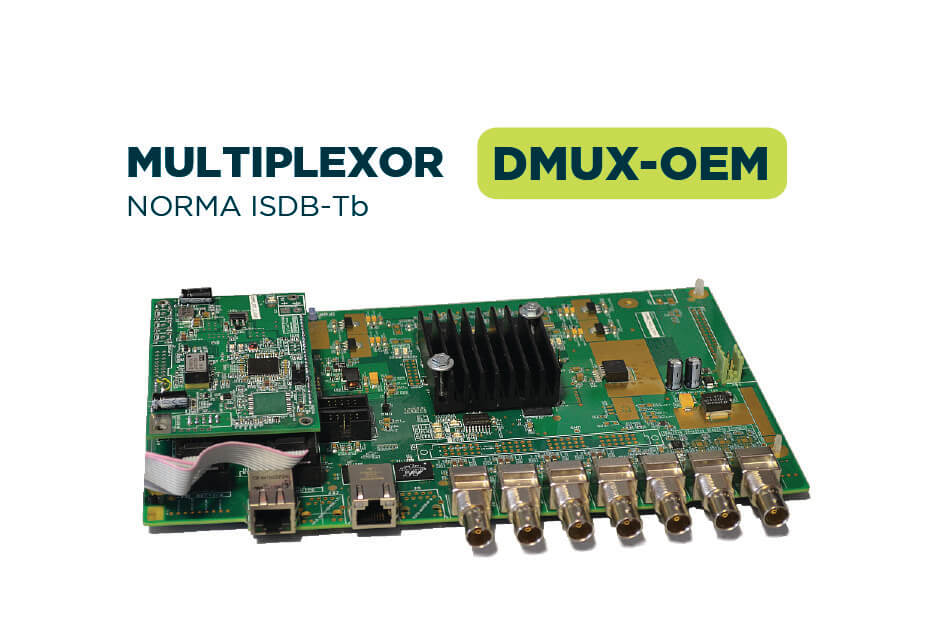
\includegraphics[width=\linewidth]{./Figures/DMUX-OEM.jpg}
        % \caption{First caption}
        % \label{fig:vs-mux}
    \end{minipage}
    \hspace{.05\linewidth}
    \begin{minipage}{.45\linewidth}
        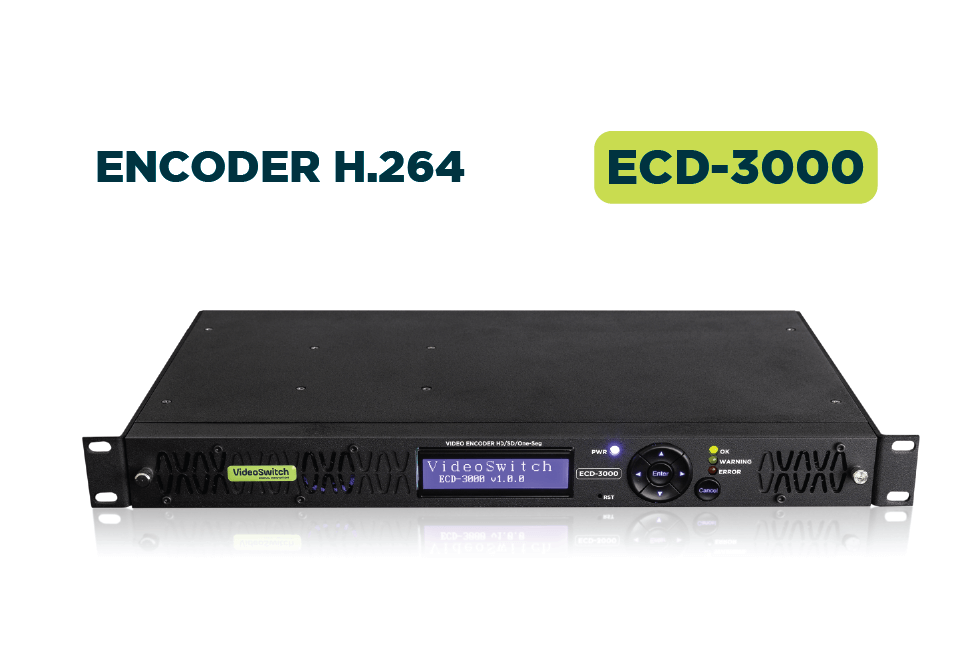
\includegraphics[width=\linewidth]{./Figures/ECD-3000.png}
        % \caption{Second caption}
        % \label{fig:vs-ecd}
    \end{minipage}
    \caption{Productos VideoSwitch, Izquierda: Multiplexor Digital - Derecha: Encoder H.264}
        \label{fig:vs-mux-ecd}
\end{figure}
\vspace{1cm}

VideoSwitch SRL \citep{vs-srl} es la empresa líder en Argentina y Hispanoamérica
en el desarrollo de equipos, soluciones y servicios para la transmisión y
acondicionamiento de video en la industria de la televisión, como por ejemplo
Multiplexor ISBD-Tb o un \textit{Encoder} H.264, Figura~\ref{fig:vs-mux-ecd},
dos productos de la marca en los que se podría implementar la solución propuesta.
Al plantear este trabajo, la empresa se encontraba vinculada a un único
fabricante de FPGAs y a una versión específica de su \textit{software} de
diseño debido a la dependencia de varios productos con un módulo propietario o
IP (del inglés \textit{Intellectual Property}) que implementaba la interfaz SDI
de la empresa proveedora. Esto implicaba la imposibilidad de aprovechar las
ventajas de programas más modernos o de otras empresas, así como la dependencia
de una sola marca de dispositivos programables. En situaciones de crisis de
disponibilidad de semiconductores, como la ocurrida durante la pandemia, se
evidencia la necesidad de que las empresas puedan independizar su producción de
un único proveedor. Por todas estas razones, el desarrollo propuesto se vuelve
estratégico para una empresa de esta envergadura.

\chapter{Introducción Específica}\label{Chapter2}

El capítulo presenta en detalle los temas aplicados en el desarrollo del trabajo y
las definiciones realizadas en el inicio del proyecto. Permite conocer los requisitos
y herramientas planteados.

\section{Requerimientos y supuestos}

  En el contexto del desarrollo de proyectos tecnológicos en el ámbito empresarial,
  es común enfrentarse a la necesidad de optimizar recursos, tanto económicos como
  técnicos. Un escenario particularmente desafiante se presenta cuando se
  identifica la oportunidad de reemplazar componentes de terceros, que suelen
  incurrir en costos de licencia significativos, por soluciones propias que no
  solo reduzcan costos sino que también ofrezcan la posibilidad de adaptación y
  mejora continua según las necesidades específicas del proyecto. Este fue
  precisamente el escenario en el que se enmarcó el desarrollo del módulo
  mientras trabajaba en la empresa VideoSwitch.

  La iniciativa para desarrollar un módulo SDI propio surgió como respuesta a la
  necesidad de contar con una solución más flexible y económicamente viable que
  los \textit{IP cores} de la empresa Altera que se estaban utilizando. Estos
  últimos, aunque funcionales, imponían limitaciones tanto en términos de costos
  como de adaptabilidad a los constantes cambios de versión de las herramientas
  de desarrollo y a la posibilidad de usar dispositivos de otras marcas, en un
  mercado con grandes problemas de abastecimiento. En este sentido, el desarrollo
  de un módulo propio se presentó no solo como una oportunidad de ahorro económico
  sino también como un desafío técnico que permitiría al equipo de
  desarrollo profundizar en el conocimiento y manejo de las interfaces de alta
  velocidad, además de ejercer un control total sobre las características y
  rendimiento del módulo.

  Para abordar este trabajo, fue necesario realizar un análisis exhaustivo de
  los requisitos técnicos y las expectativas de rendimiento que debería cumplir
  el módulo SDI\@. Este análisis implicó un trabajo colaborativo entre los
  equipos de \textit{software} y \textit{hardware} de la empresa.

  El proceso de definición de requerimientos se enfocó en capturar las
  necesidades reales de los proyectos actuales y futuros, considerando tanto
  las limitaciones técnicas inherentes al \textit{hardware} disponible como las
  oportunidades de innovación. Este enfoque permitió establecer una hoja de ruta
  clara para el desarrollo del módulo, priorizando aquellos aspectos críticos
  para el rendimiento y la funcionalidad, sin perder de vista la flexibilidad.
  Así es cómo se llegó a la siguiente lista de requerimientos.

  \begin{enumerate}
      \item Verificación
      \begin{enumerate}
          \item \textit{Tests} unitarios de cada módulo funcional.
          \item Simulación de bloques de protocolo completos.
          \item Simulación del sistema completo haciendo \textit{loopback} entre el trasmisor y el receptor.
      \end{enumerate}
      % \item Validación
      % \begin{enumerate}
      %     \item Medición y observación de audio y video luego de pasar por el sistema completo.
      %     \item Medición de los los paquetes con un analizador según la norma.
      %     \item Cumplir con el bitrate de los estándares dentro del rango de SD-SDI y 3G-SDI.
      % \end{enumerate}
      \item Funcionalidad
      \begin{enumerate}
          \item Obtener las tasas de datos contempladas dentro del rango de las normas SD-SDI y 3G-SDI\@.
          \item Obtener un diseño sin problemas de \textit{timing} en las señales entre dominios de reloj
          dentro del módulo.
          \item Obtener un módulo sin problemas de \textit{timing} por \textit{setup} o \textit{hold} en las señales de entrada y salida.
          \item La implementación del sistema no debe ocupar más de 3000 \textit{Logic Array Blocks} en la FPGA\@.
      \end{enumerate}
      \item Metodología de trabajo
      \begin{enumerate}
          \item Control de versiones mediante SVN o Git.
          \item Desarrollo en Quartus con licencias para análisis de \textit{timing} y simulaciones o herramientas \textit{open source}.
          \item Planificación y documentación mediante Redmine o Gitlab.
          \item Diseño modular.
      \end{enumerate}
      \item Documentación
      \begin{enumerate}
          \item Confección de la memoria técnica.
          \item Confección de documentación del diseño del módulo.
          \item Confección de documentación de uso del módulo.
      \end{enumerate}
  \end{enumerate}

  Sin embargo, como suele ocurrir en el dinámico entorno empresarial, los cambios
  en las prioridades de gestión y mi posterior salida de la empresa llevaron a que
  casi ninguno de los supuestos planteados inicialmente para el desarrollo del
  módulo se cumpliera. Estas modificaciones en el enfoque y la asignación de
  recursos afectaron directamente la ejecución y el avance del proyecto, limitando
  la capacidad para alcanzar los objetivos propuestos con la rapidez y eficacia
  esperadas.

  A continuación, se listan los supuestos originales bajo los cuales se había
  concebido el proyecto, resaltando que, desafortunadamente, solo el último de
  estos se cumplió:

  \begin{enumerate}
      \item Se cuenta con el hardware necesario para su implementación, con driver SDI y una FPGA Cyclone V con hard-transceivers.
      \item Se cuenta con los instrumentos de medición necesarios.
      \item Se cuenta con las licencias de software necesarias para el desarrollo.
      \item Se cuenta con el módulo que se desea remplazar.
      \item Se cuenta con el tiempo necesario dentro de la empresa para hacer el desarrollo y las pruebas.
      \item Se cuenta con las normas en cuestión.
  \end{enumerate}

  El único supuesto que se logró cumplir fue el acceso a las normas pertinentes
  al desarrollo del módulo. Este ítem, aunque significativo para el entendimiento
  y la conceptualización del proyecto, resultó insuficiente para poder llegar
  con los objetivos y plazos planteados originalmente.
  
  % contrarrestar las
  % limitaciones impuestas por la no concreción de los otros supuestos necesarios
  % para un desarrollo y ejecución exitosos del módulo SDI\@.

  Esta situación refleja los retos que enfrentan los proyectos de innovación
  tecnológica en el ámbito empresarial, donde las fluctuaciones en las prioridades
  organizacionales y los cambios en los equipos de trabajo pueden alterar
  significativamente la trayectoria y los resultados de iniciativas críticas,
  subrayando la importancia de una gestión flexible y adaptativa frente a las
  inevitables dinámicas del entorno empresarial.

  Por todas estas razones, en el diseño final se decidió apostar por el uso de
  herramientas de código abierto y evitar la dependencia de hardware específico y
  propietario. Esta decisión estratégica buscaba mitigar los riesgos asociados a
  las limitaciones de \textit{hardware} y \textit{software}, permitiendo una
  mayor flexibilidad y adaptabilidad frente a los cambios y desafíos del entorno.

  El compromiso con soluciones de código abierto no solo facilita la gestión de
  recursos y la independencia tecnológica, sino que también promueve una cultura
  de innovación y colaboración, esenciales para el desarrollo sostenible del
  proyecto en un contexto de incertidumbre y cambio constante.

\section{Nociones básicas del sistema}

  \subsection{Formato de datos}

  En aplicaciones SD y ED, el formato de datos serie se define con un ancho de 10 bits,
  mientras que en aplicaciones HD es de 20 bits, divididos en dos flujos de datos paralelos
  de 10 bits cada uno (conocidos como Y y C). El flujo de datos SD se organiza de la
  siguiente manera:

  \begin{verbatim}
  Cb Y Cr Y' Cb Y Cr Y'
  \end{verbatim}

  Mientras que los flujos de datos HD se organizan así:

  \begin{verbatim}
  Y
  Y Y' Y Y' Y Y' Y Y'
  C
  Cb Cr Cb Cr Cb Cr Cb Cr
  \end{verbatim}

  Para todas las interfaces digitales serie (excluyendo las codificaciones compuestas
  obsoletas), la codificación de color nativa es el formato YCbCr 4:2:2. El canal de
  luminancia (Y) se codifica con un ancho de banda completo (13,5 MHz en SD de 270 Mbit/s,
  ~75 MHz en HD), y los dos canales de crominancia (Cb y Cr) se submuestrean horizontalmente
  y se codifican con la mitad de ancho de banda (6,75 MHz o 37,5 MHz). Las muestras Y, Cr y
  Cb están co-situadas (adquiridas en el mismo instante de tiempo), y la muestra Y' se
  adquiere en el momento intermedio entre dos muestras Y adyacentes.

  En lo anterior, Y se refiere a muestras de luminancia, y C a muestras de crominancia. Cr y
  Cb se refieren además a los canales de diferencia de color rojo y azul; ver vídeo por
  componentes para más información. Esta sección solo discute la codificación de color nativa
  de SDI\@; otras codificaciones de color son posibles tratando la interfaz como un canal de
  datos de 10 bits genérico. El uso de otras codificaciones de colorimetría, y la conversión
  a y desde el espacio de color RGB, se discute a continuación.

  La carga útil de vídeo (así como la carga útil de datos auxiliares) puede usar cualquier
  palabra de 10 bits en el rango de 4 a 1019 (004\textsubscript{16} a 3FB\textsubscript{16})
  inclusive; los valores 0–3 y 1020–1023 (3FC\textsubscript{16}–3FF\textsubscript{16}) están
  reservados y no pueden aparecer en ninguna parte de la carga útil. Estas palabras reservadas
  tienen dos propósitos; se utilizan tanto para paquetes de sincronización como para cabeceras
  de datos auxiliares.

  \subsection{Paquetes de sincronización}

  Un paquete de sincronización (comúnmente conocido como la señal de referencia de tiempo o TRS)
  ocurre inmediatamente antes de la primera muestra activa en cada línea, e inmediatamente después
  de la última muestra activa (y antes del inicio de la región de borrado horizontal). El paquete
  de sincronización consta de cuatro palabras de 10 bits, las primeras tres palabras siempre son
  las mismas: 3FF\textsubscript{16}, 0, 0; la cuarta consta de 3 bits de bandera, junto con un código de corrección
  de errores. Como resultado, hay 8 paquetes de sincronización diferentes posibles.

  En las interfaces HD-SDI y de enlace dual, los paquetes de sincronización deben
  ocurrir simultáneamente en ambos flujos de datos Y y C (se permite cierto retraso
  entre ambos, con tal fin el equipo debe ser capaz de almacenar en búfer adelantado
  para que se sincronicen). En interfaces SD-SDI y de definición mejorada, solo
  hay un flujo de datos, y por lo tanto, solo un paquete de sincronización a la
  vez. Aparte del tema de cuántos paquetes aparecen, su formato es el mismo en
  todas las versiones de la interfaz digital-serial.

  Los bits de bandera encontrados en la cuarta palabra (comúnmente conocida como la palabra XYZ)
  son conocidos como H, F y V. El bit H indica el inicio del borrado horizontal; y los bits de
  sincronización que preceden inmediatamente a la región de borrado horizontal deben tener H
  establecido en uno. Tales paquetes se conocen comúnmente como paquetes de Fin de Vídeo Activo, o
  paquetes EAV\@. De manera similar, el paquete que aparece inmediatamente antes del inicio del vídeo
  activo tiene H establecido en 0; este es el paquete de inicio de vídeo activo o paquete SAV\@.

  De manera similar, el bit V se utiliza para indicar el inicio de la región de borrado vertical; un
  paquete EAV con V=1 indica que la siguiente línea (las líneas se consideran que comienzan con el
  paquete SAV) será la primera línea del borrado vertical. De manera similar, un paquete SAV con V=1
  indica que la línea actual es la primera línea del vídeo activo después del borrado vertical. Los
  paquetes SAV/EAV con V=0 indican líneas dentro de la región de vídeo activo, o dentro de la región
  de borrado horizontal, pero no el inicio o el final de ninguna de estas regiones.

  El bit F se utiliza para distinguir entre campos en formatos entrelazados o segmentados
  progresivamente. En formatos progresivos, F siempre es 0. En formatos entrelazados o segmentados
  progresivamente, F es 0 para todas las líneas en el primer campo o segmento, y 1 para todas las
  líneas en el segundo campo o segmento. La designación de cuál de los dos campos o segmentos se
  considera el primero es arbitraria.

\section{Estructura general del sistema y diagrama en bloques}

  En cuanto a la implementación en FPGA, la interfaz SDI consta de dos capas
  independientes, que se pueden visualizar en la figura~\ref{fig:sdi1}, la de
  recepción/transmisión y la de protocolo, por tal motivo el módulo deberá
  implementar ambas instancias de manera separada. Para la primera, se suelen
  usar \textit{hard-transceivers}, contenidos en la FPGA o \textit{soft-transceivers}
  instanciados en la lógica programable, para las aplicaciones con menor demanda
  de tasa de datos. Este módulo se puede encargar de muestrear la entrada
  asincrónica, sincronizarse a la misma y deserializar los datos, para casos más
  exigentes es necesario usar un \textit{hard-transceivers}. En este diseño no se
  pretende resolver esta parte del desarrollo, sino usar las soluciones que
  proporcionan los fabricantes de los dispositivos, que por lo general son de uso
  libre, aunque propietarias. El desarrollo que puede ser necesario dependiendo
  el fabricante que se elija es el controlador de dicho módulo.

  Para la segunda etapa, se debe implementar un submódulo que trabaje en el dominio
  de los datos paralelizados y tenga la información propia del protocolo para
  interpretar, acondicionar y validar la señal. Esta parte del desarrollo se
  encarga principalmente de la sincronización de paquetes y de la detección de
  errores. Aunque la interfaz funciona en un solo sentido a la vez, debe ser
  configurable para funcionar como transmisor y receptor de manera separada, como
  se ilustra en la figura~\ref{fig:sdi1}. Por lo tanto, el módulo debe ser capaz
  de tomar la señal serie que llega a la FPGA desde el \textit{driver} del cable,
  deserializarla y procesarla en un sentido y empaquetarla (acorde al
  protocolo) y serializarla en el otro sentido.

  \begin{figure}[htbp]
      \centering
      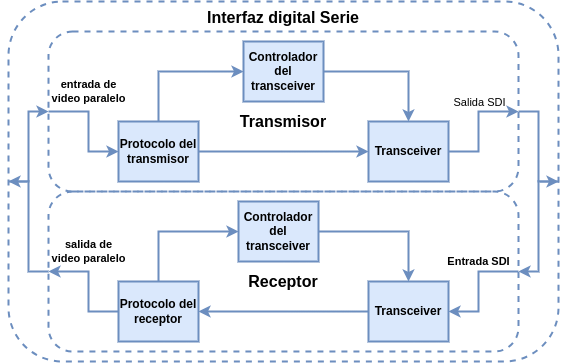
\includegraphics[width=\linewidth]{./Figures/sdi.png}
      \caption{Diagrama en bloques general de interfaz digital serie.}\label{fig:sdi1}
  \end{figure}

\section{Estándares soportados por la interfaz}

  El módulo soporta SMPTE SD/HD/3G-SDI implementa tres estándares de la interfaz:

  \begin{itemize}
      \item SD-SDI (SMPTE ST 259): señal digital de televisión estándar~\citep{st259}.
      \item HD-SDI (SMPTE ST 292\-1): interfaz serie de señal de 1,5 Gb/s~\citep{st292}.
      \item 3G-SDI (SMPTE ST 424): interfaz serie de señal de 3 Gb/s~\citep{st424}.
  \end{itemize}

  \subsection{Definición estándar}

  El módulo está diseñado para soportar la tasa de bits de 270 Mb/s y es compatible
  con el estándar de detección y manejo de errores o EDH (del inglés, \textit{Error
  Detection and Handling}) SMPTE RP 165~\citep{st165} para las secciones de
  recepción y transmisión~\citep{castr}.

  \subsection{Alta definición}

  Aunque el estándar se llama interfaz de 1,5 Gb/s, las tasas de bits admitidas
  por HD-SDI son en realidad de 1,485 Gb/s y 1,485/1,001 Gb/s. El módulo es
  compatible con ambas tasas de bits y con la generación (transmisor) y
  verificación (receptor) de valores CRC (del inglés, \textit{Cyclic Redundancy Check})
  para cada línea de video, así como la inserción (transmisor) y captura (receptor)
  de valores de número de línea para cada línea~\citep{castr}.

  \subsection{Ultra alta definición}

  Como con el estándar anterior, llama interfaz de 3 Gb/s, pero las tasas de bits
  real son de 2,97 Gb/s y 2,97/1,001 Gb/s. El módulo es compatible con ambas tasas
  de bits. 3G-SDI admite varios niveles de mapeo diferentes, descritos en el
  estándar SMPTE ST 425\-1. El núcleo es compatible con todos estos niveles. Al
  igual que con el estándar HD-SDI, el núcleo también es compatible con la
  generación y verificación de CRC, así como la inserción y captura de números de
  línea para 3G-SDI\@~\citep{castr}.

  \subsection{Identificación de carga útil y soporte de datos auxiliares}

  El módulo implementa una capacidad de inserción de paquetes de datos auxiliares
  de identificación de carga útil SMPTE ST 352~\citep{st352} para el transmisor que funciona en
  todos los 3 modos SDI ya mencionados. El lado receptor también detecta y captura
  los cuatro bytes de datos de los paquetes de identificación de carga útil ST 352.

  Además, implementa la inserción de paquetes de datos auxiliares antes de la
  transmisión. Aunque el módulo no proporciona una capacidad de inserción de paquetes
  de datos auxiliares, excepto para los paquetes de identificación de carga útil
  ST 352~\citep{st352}, tiene puertos de datos necesarios para permitir que la inserción de
  paquetes de datos auxiliares sea implementada por el usuario. En el lado del
  receptor, todos los datos auxiliares insertados son preservados por el receptor.
  El módulo pueden procesar el flujo de datos SDI recibidos y/o modificar los datos
  auxiliares según sea necesario~\citep{design}.

\section{Simulación y verificación}

  La verificación y validación de código y modelos por medio de simulación es
  un aspecto crucial para garantizar calidad y reducir tiempos de desarrollo,
  sobre todo en sistemas críticos. La verificación garantiza con simulaciones y
  permite la corrección del código, antes de hacer pruebas en el mundo real, que
  son más lentas y costosas. La validación se relaciona con la conexión del
  desarrollo con el mundo real y su uso previsto, implica contar con el
  \textit{hardware} y el instrumental de medición. Además, en sistemas de alta
  complejidad la simulación permite probar cada módulo por separado, técnica que
  facilita la integración y permite distinguir con claridad los errores, lo que
  acelera proceso de aprendizaje y comprensión del sistema. Por otro lado al ser
  capaces de simular datos de cierto modelo, se garantiza que uno entiende el
  modelo, sus restricciones y limitaciones~\citep{testbench}.

  \begin{figure}[htbp]
      \centering
      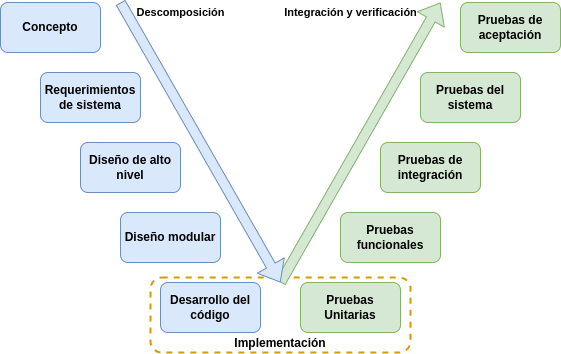
\includegraphics[width=\linewidth]{./Figures/verif.png}
      \caption{Diagrama pasos a seguir para diseñar, implementar y verificar un proyecto.}\label{fig:verif}
  \end{figure}

  % En este trabajo se llevaron a cabo test unitarios para cada módulo básico del
  % desarrollo e incluso aquellos que integraban varios submódulos, usando GHDL,
  % cocotb e integración continua en Github, pero para la verificación del sistema
  % completo fue necesario usar Quartus y ModelSim, ya que no se contaba con los
  % modelos de los Transceivers debido a que son herramientas propietarias.

  Las pruebas unitarias son a nivel de código y ayudan a eliminar
  problemas en una etapa temprana, principalmente el desarrollador es responsable
  de realizarla para su código.

  Las pruebas funcionales están asociadas con la fase de diseño de bajo nivel
  que garantiza que los módulos de códigos y unidades estén trabajando correctamente
  para ejecutar nuevas funciones o servicios.

  Las pruebas de integración están asociadas con la fase de diseño de alto
  nivel. Estas garantizan la integración entre todos los módulos del sistema después
  de agregar nuevas funciones o actualizaciones.

  Las pruebas de sistema están asociados con los requisitos y la fase de
  diseño del sistema. Combinan el \textit{software}, el \textit{hardware} y la
  integración de este sistema con otros sistemas externos.

  Las pruebas de aceptación del usuario están asociadas con la fase de
  análisis empresarial y operativo. Los usuarios clientes son los principales
  ejecutores de esta prueba basada en casos de prueba y escenarios que cubren los
  requisitos comerciales para garantizar que se haya entregado el producto correcto
  según las especificaciones.

  Dado que, durante la implementación de este desarrollo, no se disponía del
  equipamiento de la empresa VideoSwitch, se enfocó especialmente en las etapas
  iniciales. Se llevaron a cabo pruebas a nivel del sistema de manera parcial,
  omitiendo las pruebas de aceptación~\citep{testbench}.

  % Debido a que al momento de la ejecución de este desarrollo no se sigue contando
  % con el equipamiento de la empresa VideoSwitch, se puso especial énfasis en las
  % primeras etapas, ejecutando Las pruebas a nivel sistema solo de forma
  % parcial y dejando de lado Las pruebas de aceptación.

\section{Integración continua}

La integración continua o CI (del inglés, \textit{continuous integration}) es una
práctica que nace de la ingeniería de software, pero que en los últimos años se
a ido extendiendo a otras ramas de la ingeniería, que consiste en hacer
integraciones automáticas de un proyecto con cierta regularidad para así poder
detectar errores cuanto antes. Se entiende por integración la compilación o
síntesis y ejecución de pruebas de un proyecto completo y sus subsistemas. 

Por lo general se necesita un sistema de control de versiones que acompañe y
ejecute el proceso de CI\@. Los mismos también se complementan con otras
comprobaciones como las pruebas automatizadas de calidad del código, las
herramientas de revisión de estilo de sintaxis, entre otras.

Los beneficios comúnmente citados de la integración continua incluyen:
\begin{itemize}
  \item Detección temprana y mejorada de errores, y métricas que le permiten
  abordar los errores a tiempo, a veces tras solo unos minutos de la incorporación.
  \item Progreso continuo y demostrado para mejorar la retroalimentación.
  \item Mejor colaboración en equipo: todos los miembros del equipo pueden 
  cambiar el código, integrar el sistema y determinar rápidamente los conflictos
  con otras partes de este.
  \item Integración mejorada del sistema, lo que reduce las sorpresas al final
  del ciclo de vida del desarrollo.
  \item Menos cambios paralelos para la fusión y prueba.
  \item Reducción de cantidad de errores durante las pruebas del sistema.
  \item Sistemas actualizados constantemente en los que realizar las pruebas.
\end{itemize}

Para este trabajo se optó por usar Git como sistema de control de
versiones, más específicamente GitHub, que con GitHub Actions también entrega
la funcionalidad de integración continua~\citep{cicd}.
\chapter{Diseño e Implementación}
\label{Chapter3}

\section{Req}

% \input{example}

\section{Infraestructura para el Desarrollo}

\subsection{Simulación}

\subsubsection{¿Qué es \textit{cocotb}?}
\textit{cocotb} (por sus siglas en inglés \textit{COroutine based COsimulation TestBench}) es
un entorno de \textit{TestBench} de verificación de simulación basado en
corrutinas para verificar RTL (por sus siglas en inglés \textit{Register Transfer Level})
descriptos en VHDL y SystemVerilog utilizando Python.

Este \textit{Framework} es completamente gratuito, de código abierto (Licencia
BSD) y alojado en GitHub.\textit{cocotb} requiere un simulador para simular el
diseño HDL (por sus siglas en inglés \textit{Hardware Description Language}) y se puede
utilizar con una variedad de simuladores en multiples sistemas operativos.

\textit{cocotb} fomenta la filosofía de reutilización de diseño y pruebas
aleatorias que UVM, sin embargo, está implementado en Python.

Con \textit{cocotb}, los HDL tradicionales se utilizan solo para el diseño en
sí, no para el banco de pruebas. Además, tiene soporte incorporado para
integrarse con sistemas de integración continua y fue diseñado específicamente
para reducir la sobrecarga de la creación de una prueba.También descubre
automáticamente las pruebas, por lo que no se requiere un paso adicional para
agregar una prueba a una regresión.

La verificación se realiza integramente con Python, lo cual tiene varias
ventajas por sobre el uso de SystemVerilog o VHDL para la verificación:

\begin{itemize}
  \item Es rápido escribir en Python, es un lenguaje muy productivo.
  \item Es fácil interfacear con otros lenguajes.
  \item Python tiene una enorme biblioteca de código existente para reutilizar.
  \item Python es interpretado: las pruebas se pueden editar y volver a ejecutar
  sin tener que recompilar el diseño.
  \item Python es popular: muchos más desarrolladores conocen Python que
  SystemVerilog o VHDL.
\end{itemize}

\subsubsection{¿Cómo funciona \textit{cocotb}?}

Un banco de pruebas típico de \textit{cocotb} no requiere código RTL adicional.
El Diseño Bajo Prueba (DUT, por sus siglas en inglés \textit{Design-Device
under Test}) se instancía como el \textit{toplevel} en el simulador sin ningún
código que haga de interfaz o \textit{wrapper}.\textit{cocotb} proporciona
estímulos a las entradas del DUT (o incluso más abajo en la jerarquía) y
supervisa las salidas directamente desde Python.

\begin{figure}[h]
  \centering
  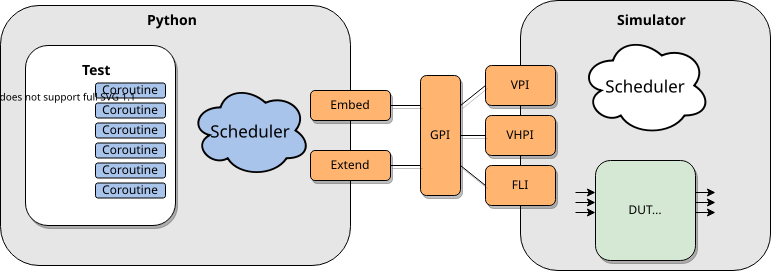
\includegraphics[width=0.7\textwidth]{./Figures/cocotb_overview.png}
  \caption{Visión general de \textit{cocotb}.}
\end{figure}

% Una prueba es simplemente una función Python. En cualquier momento, el simulador
% está avanzando en el tiempo o el código Python se está ejecutando. La palabra
% clave \texttt{await} se utiliza para indicar cuándo pasar el control de
% ejecución de vuelta al simulador. Una prueba puede generar múltiples corutinas,
% lo que permite flujos de ejecución independientes.

\subsection{CI-CD}

\section{Estructura General del Sistema}

\section{{Planificación}}

% \chapter{Ensayos y Resultados}
\label{Chapter4}

% \section{Infraestructura para el Desarrollo}

\section{Simulación y Verificación}

La verificación y validación de código y modelos por medio de simulación es
un aspecto crucial para garantizar calidad y reducir tiempos de desarrollo,
sobre todo en sistemas críticos. La verificación garantiza con simulaciones y
permite la corrección del código, antes de hacer pruebas en el mundo real, que
son más lentas y costosas. La validación se relaciona con la conexión del
desarrollo con el mundo real y su uso previsto, implica contar con el
\textit{hardware} y el instrumental de medición. Además, en sistemas de alta
complejidad la simulación permite probar cada módulo por separado, técnica que
facilita la integración y permite distinguir con claridad los errores, lo que
acelera proceso de aprendizaje y comprensión del sistema. Por otro lado al ser
capaces de simular datos de cierto modelo, se garantiza que uno entiende el
modelo, sus restricciones y limitaciones.

% En este trabajo se llevaron a cabo test unitarios para cada módulo básico del
% desarrollo e incluso aquellos que integraban varios submódulos, usando GHDL,
% cocotb e integración continua en Github, pero para la verificación del sistema
% completo fue necesario usar Quartus y ModelSim, ya que no se contaba con los
% modelos de los Transceivers debido a que son herramientas propietarias.

\subsection{\textit{cocotb}}
\textit{cocotb} (por sus siglas en inglés \textit{COroutine based COsimulation
TestBench}) es un entorno de \textit{TestBench} de verificación de simulación
basado en corrutinas para verificar RTL (por sus siglas en inglés
\textit{Register Transfer Level}) descriptos en VHDL y SystemVerilog utilizando
Python.

Este \textit{Framework} es completamente gratuito, de código abierto (Licencia
BSD) y alojado en GitHub.\textit{cocotb} requiere un simulador para simular el
diseño HDL (por sus siglas en inglés \textit{Hardware Description Language}) y
se puede utilizar con una variedad de simuladores en multiples sistemas
operativos.

\textit{cocotb} fomenta la filosofía de reutilización de diseño y pruebas
aleatorias que UVM, sin embargo, está implementado en Python.

Con \textit{cocotb}, los HDL tradicionales se utilizan solo para el diseño en
sí, no para el banco de pruebas. Además, tiene soporte incorporado para
integrarse con sistemas de integración continua y fue diseñado específicamente
para reducir la sobrecarga de la creación de una prueba.También descubre
automáticamente las pruebas, por lo que no se requiere un paso adicional para
agregar una prueba a una regresión.

La verificación se realiza integramente con Python, lo cual tiene varias
ventajas por sobre el uso de SystemVerilog o VHDL para la verificación:

\begin{itemize}
  \item Es rápido escribir en Python, es un lenguaje muy productivo.
  \item Es fácil interfacear con otros lenguajes.
  \item Python tiene una enorme biblioteca de código existente para reutilizar.
  \item Python es interpretado: las pruebas se pueden editar y volver a ejecutar
  sin tener que recompilar el diseño.
  \item Python es popular: muchos más desarrolladores conocen Python que
  VHDL o SystemVerilog.
\end{itemize}

\subsection{Funcionamiento de \textit{cocotb}}

Un banco de pruebas típico de \textit{cocotb} no requiere código RTL adicional.
El Diseño Bajo Prueba (DUT, por sus siglas en inglés \textit{Design-Device
under Test}) se instancía como el \textit{toplevel} en el simulador sin ningún
código que haga de interfaz o \textit{wrapper}.\textit{cocotb} proporciona
estímulos a las entradas del DUT (o incluso más abajo en la jerarquía) y
supervisa las salidas directamente desde Python.

\begin{figure}[h]
  \centering
  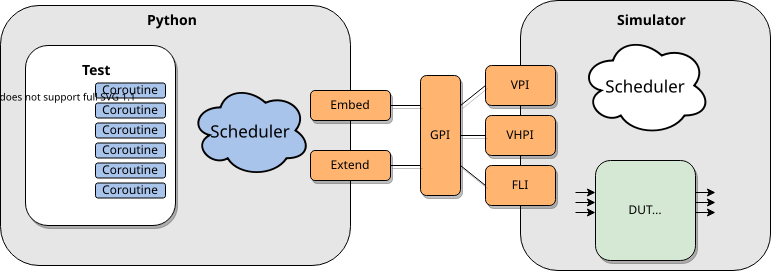
\includegraphics[width=0.7\textwidth]{./Figures/cocotb_overview.png}
  \caption{Visión general de \textit{cocotb}.}
\end{figure}

% Una prueba es simplemente una función Python. En cualquier momento, el simulador
% está avanzando en el tiempo o el código Python se está ejecutando. La palabra
% clave \texttt{await} se utiliza para indicar cuándo pasar el control de
% ejecución de vuelta al simulador. Una prueba puede generar múltiples corutinas,
% lo que permite flujos de ejecución independientes.

\subsection{Estructura Genérica de los \textit{Test} y sus resultados}

\section{Integración Continua}

La integración continua (CI, del inglés \textit{continuous integration}) es una
práctica que nace de la ingeniería de software, pero que en los últimos años se
a ido extendiendo a otras ramas de la ingeniería, que consiste en hacer
integraciones automáticas de un proyecto con cierta regularidad para así poder
detectar errores cuanto antes. Se entiende por integración la compilación o
síntesis y ejecución de pruebas de un proyecto completo y sus subsistemas. 

Por lo general se necesita un sistema de control de versiones que acompañe y
ejecute del proceso de CI\@. Los mismos también se complementan con otras
comprobaciones como las pruebas automatizadas de calidad del código, las
herramientas de revisión de estilo de sintaxis, entre otras.

Para pasar en limpio, los beneficios comúnmente citados de la integración
continua incluyen:
\begin{itemize}
  \item Detección temprana y mejorada de errores, y métricas que le permiten
  abordar los errores a tiempo, a veces tras solo unos minutos de la incorporación.
  \item Progreso continuo y demostrado para mejorar la retroalimentación.
  \item Mejor colaboración en equipo: todos los miembros del equipo pueden.
  cambiar el código, integrar el sistema y determinar rápidamente los conflictos
  con otras partes del del mismo.
  \item Integración mejorada del sistema, lo que reduce las sorpresas al final
  del ciclo de vida del desarrollo.
  \item Menos cambios paralelos para la fusión y prueba.
  \item Reducción de cantidad de errores durante las pruebas del sistema.
  \item Sistemas actualizados constantemente en los que realizar las pruebas.
\end{itemize}

En el caso de este trabajo se optó por usar Git como sistema de control de
versiones, más específicamente Github, que con Github Actions también entrega
la funcionalidad de integración continua.

% \section{Quartus y ModelSim}

\section{Resultados}

\subsection{Resultados Generales}

\subsection{Resultados por módulo}

% \chapter{Conclusiones}\label{Chapter5}

El capítulo final muestra los resultados alcanzados con el trabajo e informa las
mejoras necesarias a futuro.

\section{Resultados obtenidos}

% El funcionamiento del dispositivo es el esperado.
% La cantidad de recursos utilizados es la esperada. 
% Es mejor usar software abierto.
% La implementación de test mediante python, pytest y cocotb facilito mucho el desarrollo.
% El CI ayudo a encontrar problema que surgian en algún móídulo mientras se desarrollava otro.

% Hacer un desarrollo basado en una norma supuso un desafío extra

% En el desarrollo del trabajo se aplican los conocimientos adquiridos durante la
% cursada de la carrera de especialización, en particular las asignaturas de gestión
% de proyectos, Programación de microcontroladores, diseño de circuitos impresos,
% diseño para la manufacturabilidad e ingeniería de software en sistemas embebi-
% dos. El aprendizaje adquirido sobre la gestión de problemas, estructuración de
% tareas y prevención de retrasos permite finalizar la carrera con una visión com-
% pleta sobre un sistema embebido.

En el desarrollo de este trabajo, que consistió en el diseño de un módulo SDI
de triple tasa de datos para dispositivos lógicos programables, se han
alcanzado satisfactoriamente los objetivos planteados al inicio del trabajo
considerando que que solo uno de los supuestos iniciales se cumplió. El
dispositivo diseñado funciona según lo esperado, cumpliendo con las
especificaciones establecidas en la fase de diseño. Este éxito demuestra la
viabilidad del enfoque adoptado y de la funcionalidad del módulo desarrollado.

Una de las conclusiones clave de este trabajo es que la cantidad de recursos
de FPGA utilizados se alineó estrechamente con las proyecciones iniciales.
Este resultado subraya la precisión en la planificación y la eficiencia del
diseño. Además, el uso de herramientas de código abierto a lo largo de la gran
mayoría del trabajo no solo demostró ser viable, sino también preferible.
Proporcionó una mayor flexibilidad y control sobre el proceso de desarrollo,
permitiendo ajustes y modificaciones de manera ágil y eficiente, lo cual fue
crucial para el éxito del trabajo.

El proceso de implementación de pruebas, utilizando herramientas como Python,
Pytest y Cocotb, simplificó significativamente el desarrollo. Esta estrategia
facilitó una verificación eficaz y eficiente del diseño, permitiendo detectar
y corregir errores de manera temprana. La adopción de prácticas de integración
continua tuvo un rol fundamental en el mantenimiento de la integridad del
trabajo. Permitió identificar problemas que surgían en algunos módulos mientras
se desarrollaban otros, asegurando así que el trabajo avanzara de manera
cohesiva y consistente.

Abordar el diseño basándose en una normativa específica presentó desafíos
adicionales, pero también estableció un marco de referencia claro que guió el
desarrollo. Este enfoque normativo no solo aseguró la compatibilidad y el
cumplimiento del módulo SDI desarrollado, sino que también proporcionó una
estructura organizativa que facilitó el manejo de la complejidad del trabajo.
Además, la documentación de dispositivos similares fue de gran utilidad a la
resolver dudas de implementación y estructurar el flujo de datos.

Durante el desarrollo de este trabajo, se aplicaron de manera integral los
conocimientos adquiridos a lo largo de la carrera de especialización. Las
habilidades y conceptos aprendidos en temáticas como gestión de proyectos,
programación de dispositivos lógicos programables, definición de
requerimientos, especificaciones y pruebas para verificación y validación y
diseño para la reutilización y mutabilidad fueron fundamentales para el éxito
del trabajo. Esta aplicación práctica de la teoría a un proyecto complejo y
desafiante no solo reforzó estos conocimientos, sino que también proporcionó
una experiencia enriquecedora.

Finalmente, este trabajo no solo cumplió con la gran mayoría de los objetivos
técnicos propuestos, sino que también sirvió como una valiosa experiencia de
aprendizaje. Demostró la importancia de combinar la teoría con la práctica en
el campo de la ingeniería y subrayó el valor de un enfoque metodológico y
reflexivo en el desarrollo de soluciones tecnológicas avanzadas. Este trabajo
prepara el terreno para futuras investigaciones y desarrollos.

\section{Trabajo futuro}

% Llevar el modulo hasta los estandares de 12G.
% Terminar de testear los formatos restantes.
% Agregar formal verification a los módulos.
% Implementar los test funcionales en UVM para que el testeo sea estandar.
% Probar en los equipos de la empresa VideoSwitch.
% Hacer mediciones con equipamiento específico para los estandares y con capacidad de análizar la integridad de la señal de TV.

Mirando hacia el futuro, existen varias áreas en las que el trabajo podría
expandirse y mejorar. Uno de los objetivos principales sería llevar el módulo
hasta los estándares de 12G, lo que ampliaría significativamente su aplicabilidad
y permitiría su uso en una gama más amplia de aplicaciones de alta velocidad.
Además, sería crucial terminar de probar los formatos restantes para asegurar
una compatibilidad y funcionalidad completas del módulo en diferentes escenarios
de uso.

La adición de verificación formal a los módulos representaría un paso adelante
en el aseguramiento de la calidad y la confiabilidad del diseño. Esta
metodología puede ayudar a identificar problemas que no son fácilmente
detectables mediante pruebas convencionales. Implementar las pruebas funcionales
en UVM (del inglés, \textit{Universal Verification Methodology}) estándarizaría el
proceso de verificación, facilitando la reutilización de los \textit{test} y
mejorando la eficiencia del proceso de verificación. Se plantea el uso de PyUVM,
que se integra perfectamente con Cocotb, presenta todas las funcionalidades de
UVM en SystemVerilog, pero al estar basado en Python agiliza el desarrollo.

Además, sería valioso probar el módulo en equipos específicos de la empresa
VideoSwitch, lo que proporcionaría una validación final del diseño en un entorno
de producción real. Por último, realizar mediciones con equipamiento específico
para los estándares y con capacidad de analizar la integridad de la señal de
televisión sería esencial para garantizar que el módulo cumple con los requisitos
de calidad y rendimiento más exigentes.


%   CONTENIDO DE LA MEMORIA  - APÉNDICES

% \appendix % indicativo para indicarle a LaTeX los siguientes "capítulos" son apéndices

% Incluir los apéndices de la memoria como archivos separadas desde la carpeta Appendices
% Descomentar las líneas a medida que se escriben los apéndices

% % Appendix A
% \newpage
% \KOMAoptions{paper=landscape,pagesize}
% \recalctypearea
% \begin{sidewaysfigure}
\chapter{Template de carpetas y archivos} % Main appendix title
\label{AppendixA} % For referencing this appendix elsewhere, use \ref{AppendixA}

\definecolor{mygreen}{rgb}{0,0.6,0}
\definecolor{mygray}{rgb}{0.5,0.5,0.5}
\definecolor{mymauve}{rgb}{0.58,0,0.82}

\lstset{ %
  backgroundcolor=\color{white},   % choose the background color; you must add \usepackage{color} or \usepackage{xcolor}
  basicstyle=\footnotesize,        % the size of the fonts that are used for the code
  breakatwhitespace=false,         % sets if automatic breaks should only happen at whitespace
  breaklines=true,                 % sets automatic line breaking
  captionpos=b,                    % sets the caption-position to bottom
  commentstyle=\color{mygreen},    % comment style
  deletekeywords={...},            % if you want to delete keywords from the given language
  %escapeinside={\%*}{*)},          % if you want to add LaTeX within your code
  %extendedchars=true,              % lets you use non-ASCII characters; for 8-bits encodings only, does not work with UTF-8
  %frame=single,	                % adds a frame around the code
  keepspaces=true,                 % keeps spaces in text, useful for keeping indentation of code (possibly needs columns=flexible)
  keywordstyle=\color{blue},       % keyword style
  language=[ANSI]C,                % the language of the code
  %otherkeywords={*,...},           % if you want to add more keywords to the set
  numbers=left,                    % where to put the line-numbers; possible values are (none, left, right)
  numbersep=5pt,                   % how far the line-numbers are from the code
  numberstyle=\tiny\color{mygray}, % the style that is used for the line-numbers
  rulecolor=\color{black},         % if not set, the frame-color may be changed on line-breaks within not-black text (e.g. comments (green here))
  showspaces=false,                % show spaces everywhere adding particular underscores; it overrides 'showstringspaces'
  showstringspaces=false,          % underline spaces within strings only
  showtabs=false,                  % show tabs within strings adding particular underscores
  stepnumber=1,                    % the step between two line-numbers. If it's 1, each line will be numbered
  stringstyle=\color{mymauve},     % string literal style
  tabsize=2,	                   % sets default tabsize to 2 spaces
  title=\lstname,                  % show the filename of files included with \lstinputlisting; also try caption instead of title
  morecomment=[s]{/*}{*/}
}

Se presenta la estructura de archivos con tres subcarpetas para cada módulo, como hdl, model y test, ofrece varias ventajas significativas en el desarrollo de software.

\begin{figure}[h]
  \centering
  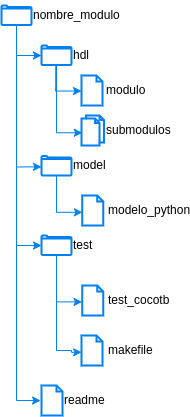
\includegraphics[width=0.5\textwidth]{./Figures/files.png}
  \caption{Estructura de carpetas.}\label{fig:files}
\end{figure}

Dividir los archivos en subcarpetas específicas para el código del módulo, los modelos de referencia y las pruebas facilita la organización y la navegación del proyecto. Esto hace que sea más fácil para los desarrolladores encontrar y comprender rápidamente los diferentes aspectos del módulo.

Al separar claramente el código del módulo, los modelos de referencia y las pruebas, se simplifica el proceso de mantenimiento. Los cambios en el código del módulo no afectarán los modelos de referencia o las pruebas, lo que permite realizar actualizaciones de manera más eficiente y reducir el riesgo de introducir errores.

La separación de los modelos de referencia del código del módulo facilita la reutilización de código. Los modelos de referencia pueden ser utilizados por otros módulos o proyectos, lo que ayuda a evitar la duplicación de esfuerzos y promueve la consistencia en el desarrollo.

La estructura organizativa clara y coherente facilita la colaboración entre varios desarrolladores en un proyecto. Cada desarrollador puede trabajar en diferentes aspectos del módulo de manera simultánea sin interferir con el trabajo de los demás, lo que mejora la eficiencia y la productividad del equipo.

El siguiente archivo presenta un ejemplo de uno de los módulos:


\begin{lstlisting}[caption= "Submódulo VHDL de ejemplo"]
  library ieee;
  use ieee.std_logic_1164.all;

  entity crc18 is
    generic(
      DATA_W : positive := 10;
      POLY_ORDER  : positive := 18
    );
    port (
      clk       : in  std_logic;                      -- 74.25 MHz
      rst       : in  std_logic;                      -- async
      clk_en    : in  std_logic;
      crc_en    : in  std_logic;
      crc_clr   : in  std_logic;
      data_i    : in  std_logic_vector(DATA_W-1 downto 0);
      crc_o     : out std_logic_vector(POLY_ORDER-1 downto 0)
    );
  end crc18;

  architecture rtl of crc18 is

    signal temp     : std_logic_vector(DATA_W-1 downto 0);
    signal crc_new  : std_logic_vector(POLY_ORDER-1 downto 0);
    signal crc_old  : std_logic_vector(POLY_ORDER-1 downto 0);
    signal crc_reg  : std_logic_vector(POLY_ORDER-1 downto 0)
                      := (others => '0');

  begin

    crc_old <= (others => '0') when crc_clr = '1' else crc_reg;

    in_xor_p: process(data_i, crc_old)
    begin
      for i in 0 to DATA_W-1 loop
          temp(i) <= data_i(i) xor crc_old(i);
      end loop;
    end process;

    crc_p: process (crc_old, temp)
    begin
      for i in 0 to 2 loop
        crc_new(i) <= crc_old(i + 10);
      end loop;
      crc_new(3) <= temp(0) xor crc_old(13);
      for i in 4 to 7 loop
        crc_new(i) <= (temp(i - 3) xor temp(i - 4)) xor
                      crc_old(i + 10);
      end loop;
      for i in 8 to 12 loop
        crc_new(i) <= (temp(i - 3) xor temp(i - 4)) xor
                      temp(i - 8);
      end loop;
      crc_new(13) <= temp(9) xor temp(5);
      for i in 14 to POLY_ORDER-1 loop
        crc_new(i) <= temp(i - 8);
      end loop;
    end process;

    out_reg_p: process(clk, rst)
    begin
      if (rst = '1') then
        crc_reg <= (others => '0');
        crc_o   <= (others => '0');
      elsif (rising_edge(clk)) then
        if (clk_en = '1') then
          if (crc_en = '1') then
            crc_reg <= crc_new;
            crc_o   <= crc_new;
          end if;
        end if;
      end if;
    end process;

  end rtl;
\end{lstlisting}

El siguiente archivo presenta un ejemplo de un submódulo:


\begin{lstlisting}[caption= "Módulo VHDL de ejemplo"]
  library ieee;
  use ieee.std_logic_1164.all;

  entity crc_insert is
    generic(
      DATA_W      : positive := 10;
      POLY_ORDER  : positive := 18
    );
    port(
      clk         : in  std_logic;
      rst         : in  std_logic;
      clk_en      : in  std_logic;
      d_rdy_i     : in  std_logic;
      sav         : in  std_logic;
      eav_dly     : in  std_logic;
      data_c_i    : in  std_logic_vector(DATA_W-1 downto 0);
      data_y_i    : in  std_logic_vector(DATA_W-1 downto 0);
      crc_ins_en  : in  std_logic;
      crc_word0   : in  std_logic;
      crc_word1   : in  std_logic;
      data_c_o    : out std_logic_vector(DATA_W-1 downto 0);
      data_y_o    : out std_logic_vector(DATA_W-1 downto 0)
    );
  end crc_insert;

  architecture rtl of crc_insert is

    signal crc_en       : std_logic;
    signal crc_clr      : std_logic;
    signal crc_en_rdy   : std_logic;
    signal crc_c_in     : std_logic_vector(POLY_ORDER-1 downto 0);
    signal crc_y_in     : std_logic_vector(POLY_ORDER-1 downto 0);

  begin

    crc_timing_ctrl_p: process(clk, rst)
    begin
      if (rst = '1') then
        crc_en <= '0';
        crc_clr <= '0';
      elsif (rising_edge(clk)) then
        if (clk_en = '1') then
          if (d_rdy_i = '1') then
            crc_clr <= sav;
            if (sav = '1') then
              crc_en <= '1';
            elsif (eav_dly = '1') then
              crc_en <= '0';
            end if;
          end if;
        end if;
      end if;
    end process;

    -- Instantiate the CRC generators
    crc_en_rdy <= d_rdy_i and crc_en;

    crc_y_u: entity work.crc18
    generic map(
      DATA_W      => DATA_W,
      POLY_ORDER  => POLY_ORDER
    )
    port map (
      clk     => clk,
      rst     => rst,
      clk_en  => clk_en,
      crc_en  => crc_en_rdy,
      crc_clr => crc_clr,
      data_i  => data_y_i,
      crc_o   => crc_y_in
    );

    crc_c_u: entity work.crc18
    generic map(
      DATA_W      => DATA_W,
      POLY_ORDER  => POLY_ORDER
    )
    port map (
      clk     => clk,
      rst     => rst,
      clk_en  => clk_en,
      crc_en  => crc_en_rdy,
      crc_clr => crc_clr,
      data_i  => data_c_i,
      crc_o   => crc_c_in
    );

    -- crc_insertion_p: process(all)
    crc_insertion_p: process(crc_ins_en, crc_word0, crc_word1,
                        crc_c_in, crc_y_in, data_c_i, data_y_i)
    begin
      if (crc_ins_en = '1') then
        if (crc_word0 = '1') then
          data_c_o <= (not crc_c_in(DATA_W-2) &
                      crc_c_in(DATA_W-2 downto 0));
          data_y_o <= (not crc_y_in(DATA_W-2) &
                      crc_y_in(DATA_W-2 downto 0));
        elsif (crc_word1 = '1') then
          data_c_o <= (not crc_c_in(POLY_ORDER-1) &
                      crc_c_in(POLY_ORDER-1 downto DATA_W-1));
          data_y_o <= (not crc_y_in(POLY_ORDER-1) &
                      crc_y_in(POLY_ORDER-1 downto DATA_W-1));
        end if;
      else
        data_c_o <= data_c_i;
        data_y_o <= data_y_i;
      end if;
    end process;

  end rtl;
\end{lstlisting}

El siguiente archivo presenta un ejemplo de uno de los modelos de referencia en Python:


\begin{lstlisting}[caption= "Modelo en Python de ejemplo"]
  class crc18_model:
  def __init__(self):
      self.POLY = 0b100000000001000001
      self.POLY_ORDER = 18
      self.crc_reg = 0

  def update_crc(self, data_i, crc_clr, crc_en):
      data = int(''.join(map(str, data_i)), 2)  # Convert data to an integer
      crc_old = self.crc_reg

      if crc_clr == 1:
          crc_old = 0

      temp = data ^ crc_old  # XOR data with the old CRC

      # Shift the CRC
      crc_new = (crc_old >> 1) ^ (self.POLY if (crc_old & 1) else 0)

      # Update the CRC with the XOR result
      crc_new = (crc_new & 0x1FFFF) | (temp << 17)

      if crc_en:
          self.crc_reg = crc_new

  def get_crc_output(self):
      return [1, 1, 1, 0, 0, 1, 1, 1, 0, 1, 0, 1, 1, 0, 1, 0, 0, 0]

  # # Example usage
  # simulator = crc18_model()

  # # Input data and control signals
  # data_i = [1, 0, 1, 1, 0, 0, 1, 0, 1, 1]
  # crc_clr = 0
  # crc_en = 1

  # # Update CRC based on input data and control signals
  # simulator.update_crc(data_i, crc_clr, crc_en)

  # # Get the CRC output
  # crc_output = simulator.get_crc_output()
  # print("CRC Output:", crc_output)
\end{lstlisting}

El siguiente archivo presenta un ejemplo de uno de los tests:

\begin{lstlisting}[caption= "Test de Cocotb de ejemplo"]
  import cocotb
  from cocotb import start_soon
  from cocotb.clock import Clock
  from cocotb.triggers import ClockCycles
  
  
  CLK_PERIOD = 13.47  # ns (74.25 MHz)
  DATA_W = 10
  
  
  async def init_test(dut):
      dut.rst.value = 1
      dut.clk_en.value = 1
      dut.crc_en.value = 0
      dut.crc_clr.value = 0
      start_soon(Clock(dut.clk, CLK_PERIOD, 'ns').start())
      await ClockCycles(dut.clk, 10)
      dut.rst.value = 0
      dut.crc_en.value = 1
      dut.crc_clr.value = 1
      await ClockCycles(dut.clk, 10)
  
  
  def binary_number_to_array(binary_number):
      binary_string = bin(binary_number)
      binary_string = binary_string[2:]
      binary_array = [int(bit) for bit in binary_string]
      return binary_array
  
  
  @cocotb.test()
  async def crc_basic_test(dut):
  
      model = crc18_smpte_model()
  
      input_bits = 0b1010101010
      input_vec = binary_number_to_array(input_bits)
      print(input_vec)
      model.update_crc(input_vec, dut.crc_clr.value, dut.crc_en.value)
      output_bit = model.get_crc_output()
      print(output_bit)
  
      await init_test(dut)
      print("test 3")
  
      dut.data_i.value = int(input_bits)
      dut.crc_en.value = 1
      await ClockCycles(dut.clk, 2)
      print(binary_number_to_array(dut.data_o.value))
  
      assert binary_number_to_array(dut.data_o.value)[:9] == output_bit[-9:], f"CRC consersion result is incorrect: {binary_number_to_array(dut.data_o.value)[:9]} != {output_bit[-9:]}"
  
\end{lstlisting}

El siguiente archivo presenta un ejemplo de uno de los Makefile:

\begin{lstlisting}[caption= "Makefile de ejemplo"]
  # This argument defines the simulator to be use
  SIM ?= GHDL
  # This argiment defines the language to be use
  TOPLEVEL_LANG ?= vhdl
  
  PWD=$(shell pwd)
  
  # This arguments enable the waveform generaton
  SIM_ARGS+=--wave=wave.ghw
  
  # # This arguments assign de generic value
  
  ifeq ($(TOPLEVEL_LANG),vhdl)
      VHDL_SOURCES = $(PWD)/../hdl/crc18.vhd
  else
      $(error A valid value (vhdl) was not provided for TOPLEVEL_LANG=$(TOPLEVEL_LANG))
  endif
  
  # TOPLEVEL is the name of the toplevel module in your Verilog or VHDL file
  TOPLEVEL = crc18
  
  # MODULE is the basename of the Python test file
  MODULE = test_crc18
  
  # include cocotb's make rules to take care of the simulator setup
  include $(shell cocotb-config --makefiles)/Makefile.sim
\end{lstlisting}
% \end{sidewaysfigure}
% \include{Appendices/AppendixB}

%	BIBLIOGRAPHY

\Urlmuskip=0mu plus 1mu\relax
\raggedright
\printbibliography[heading=bibintoc]

\end{document}  
